% ch07_oursystem.tex : System Design and Implementation
% Dr. Yael Mizrahi : LaTeX Technical Author
% XeLaTeX + bidi + fontspec

\selectlanguage{hebrew}

\section{תכנון המערכת וארכיטקטורת התוכנה}
\label{sec:ch07_system_design}

\subsection{ארכיטקטורת המערכת הכוללת}
\label{sec:ch07_architecture}

מערכת הניווט הביומימטית המוצעת מורכבת מארבע שכבות עיקריות: שכבת חישה, שכבת עיבוד אותות, שכבת מיזוג ואמידה, ושכבת בקרה. הארכיטקטורה מוצגת ב-\ref{fig:system_overview}. כל שכבה מתקשרת עם השכבה שמעליה ומתחתיה באמצעות ממשקים מוגדרים היטב, המאפשרים גמישות בהחלפת רכיבים והרחבה עתידית.

שכבת החישה כוללת שלושה אופני חישה עיקריים: מערך סונאר אולטראסוני עם ארבעה מתמרים בתדר 40 קילו-הרץ, חיישן IMU מסוג \en{BMI088} (6 צירים, 200 הרץ), וחיישן זרימה אופטית מסוג \en{PMW3901} (30 הרץ). כל חיישן מחובר למיקרו-בקר ייעודי המבצע עיבוד מקדים ומעביר את הנתונים לשכבת העיבוד המרכזית באמצעות פרוטוקול \en{SPI} במהירות 1 מגה-ביט לשנייה.

שכבת עיבוד האותות מריצה על מיקרו-בקר \en{Cortex-M4} בתדר 168 מגה-הרץ עם 512 קילו-בתים של זיכרון פלאש ו-128 קילו-בתים של זיכרון RAM. עיבוד אותות הסונאר כולל \en{matched filtering}, גילוי מעטפת, ואמידת דופלר באמצעות \en{pulse-pair processing}. כל אלה מבוצעים בזמן אמת בקצב 20 הרץ, עם זמן חישוב גרוע-ביותר של 2 מילישניות למחזור עיבוד מלא.

שכבת המיזוג והאמידה מממשת את מסנן קלמן המורחב (\en{EKF}) מודע-הדופלר המתואר בפרק 4, יחד עם מסנן החלקיקים ל-\en{SLAM} המתואר בפרק 5. שכבה זו רצה על אותו מיקרו-בקר \en{Cortex-M4}, תוך שימוש בספריית \en{Eigen} למטריצות ובספריית \en{ARM CMSIS-DSP} לאופטימיזציה של פעולות מתמטיות.

שכבת הבקרה מבצעת בקרת \en{PID} מדורגת (\en{cascaded PID}) בארבע רמות: מיקום (100 הרץ), מהירות (100 הרץ), גישה (250 הרץ), וקצב (500 הרץ). בקר זה צורך 8 אחוזים בלבד מכוח העיבוד של המעבד ו-4 קילו-בתים של זיכרון.

\subsection{רכיבי חומרה מפורטים}
\label{sec:ch07_hardware}

\subsubsection{מערך הסונאר האולטראסוני}
\label{sec:ch07_sonar_array}

מערך הסונאר מורכב מארבעה מתמרים פיאזואלקטריים מסוג \en{MEMS} בתדר מרכזי של 40 קילו-הרץ עם רוחב פס של 10 קילו-הרץ. המתמרים מסודרים בתצורת מערך ליניארי במרווח של 2 סנטימטרים זה מזה, המאפשר אמידת כיוון באמצעות \en{beamforming} בסיסי. כל מתמר מחובר למגבר הספק מסוג \en{class-D} המספק 1 וואט הספק שיא, ולמגבר קדמי אנלוגי בעל רעש נמוך עם הגבר של 60 דציבלים ורוחב פס של 20 קילו-הרץ.

מעגל מדידת ה-\en{time-of-flight} והדופלר משתמש בממיר זמן-דיגיטלי מסוג \en{TDC-GP22} עם רזולוציה של 22 פיקו-שניות, המאפשר אמידת טווח בדיוק של 3.8 מילימטרים. אמידת הדופלר מתבצעת באמצעות \en{pulse-pair processing} על פני 8 פולסים עוקבים, המספקת רזולוציית מהירות של 0.087 מטרים לשנייה ב-\en{SNR} של 10 דציבלים.

משקל המערכת הכולל הוא 8 גרם וצריכת ההספק היא 50 מיליוואט במהלך פעילות פעילה. המערכת פועלת בטווח טמפרטורות של 0 עד 50 מעלות צלזיוס, עם תיקון אוטומטי למהירות הקול התלויה בטמפרטורה.

\subsubsection{חיישן ה-IMU}
\label{sec:ch07_imu}

חיישן ה-\en{BMI088} הוא יחידת מדידה אינרציאלית (\en{IMU}) בעלת 6 צירים, הכוללת מד תאוצה תלת-צירי וגירוסקופ תלת-צירי. מד התאוצה פועל בטווח של ±24 ג'י עם רעש של 230 מיקרוג'י/√הרץ. הגירוסקופ פועל בטווח של ±2000 מעלות/שנייה עם רעש של 0.004 מעלות/שנייה/√הרץ. קצב הדגימה הוא 200 הרץ עבור שני החיישנים.

ה-\en{IMU} מכויל לפני כל טיסה באמצעות אלגוריתם כיוול אוטומטי המזהה ומתקן הטיות קבועות (\en{bias}) וגורמי קנה מידה (\en{scale factor}). הכיוול מתבצע במצב סטטי למשך 5 שניות, ומספק אמידת הטיות בדיוק של ±0.01 מטרים/שנייה² עבור מד התאוצה ו-±0.001 מעלות/שנייה עבור הגירוסקופ.

\subsubsection{חיישן הזרימה האופטית}
\label{sec:ch07_optical_flow}

חיישן ה-\en{PMW3901} הוא חיישן זרימה אופטית מבוסס תמונה ברזולוציה של 160x120 פיקסלים, הפועל בקצב 30 הרץ. החיישן משתמש במצלמת \en{global shutter} בשחור-לבן עם רגישות של 0.01 לוקס, המאפשרת פעולה בתנאי תאורה חלשה. אלגוריתם הזרימה האופטית \en{Lucas-Kanade} הפירמידלי מחשב מהירויות תמונה עם דיוק תת-פיקסל.

הזרימה האופטית מומרת למהירות תלת-ממדית באמצעות כיול המצלמה הידוע והגובה מהסונאר. כיול המצלמה מתבצע פעם אחת במעבדה, ומספק את מטריצת הכיול הפנימית (\en{intrinsic matrix}) ומקדמי העיוות (\en{distortion coefficients}).

\subsection{צינור עיבוד התוכנה}
\label{sec:ch07_software_pipeline}

צינור עיבוד התוכנה (\en{software pipeline}) מורכב משבעה שלבים עיקריים, המבוצעים בסדר הבא בכל מחזור עיבוד של 50 מילישניות:

\textbf{שלב 1: רכישת נתונים.} כל חיישן נקרא בקצב הדגימה שלו. נתוני ה-\en{IMU} נדגמים בקצב 200 הרץ ונאגרים בחיץ מעגלי. נתוני הסונאר נדגמים בקצב 20 הרץ. נתוני הזרימה האופטית נדגמים בקצב 30 הרץ.

\textbf{שלב 2: עיבוד מקדים.} נתוני ה-\en{IMU} עוברים תיקון הטיות וסינון מעביר-נמוך בתדר חיתוך של 50 הרץ. נתוני הסונאר עוברים \en{matched filtering}, גילוי מעטפת, ואמידת דופלר. נתוני הזרימה האופטית עוברים סינון חריגים (\en{outlier rejection}) באמצעות סף Mahalanobis.

\textbf{שלב 3: חיזוי \en{EKF}.} שלב החיזוי של ה-\en{EKF} משתמש בנתוני ה-\en{IMU} כקלט בקרה, ומפיץ את המצב והקווריאנס בקצב 200 הרץ. המודל הדינמי מבוסס על פורמליזם \en{Newton-Euler} במערכת הצירים הגופנית.

\textbf{שלב 4: תיקון \en{EKF}.} כאשר מדידות סונאר או זרימה אופטית מגיעות, שלב התיקון מעדכן את אמידת המצב. מדידות סונאר מעדכנות את הטווח והמהירות הרדיאלית. מדידות זרימה אופטית מעדכנות את המהירות הטרנסליונית.

\textbf{שלב 5: עדכון \en{SLAM}.} מסנן החלקיקים ל-\en{FastSLAM 2.0} מעודכן עם המדידות החדשות. כל חלקיק שומר השערת מסלול ואמידות נקודות ציון משלו. שיוך נתונים משתמש במרחק Mahalanobis עם מבחן סף chi-squared.

\textbf{שלב 6: זיהוי לולאות סגורות.} חתימות הד סונאר מושוות למאגר חתימות מאוחסנות. התאמות פוטנציאליות מאומתות גאומטרית באמצעות \en{RANSAC}.

\textbf{שלב 7: בקרה.} בקר ה-\en{PID} המדורג מחשב את פקודות המנוע הדרושות להשגת מסלול הייחוס.

\subsection{אינטגרציה בין רכיבים}
\label{sec:ch07_integration}

אינטגרציית הרכיבים מתבצעת באמצעות שלושה ממשקים עיקריים. ממשק החישה-עיבוד מעביר נתונים גולמיים מהחיישנים לשכבת העיבוד באמצעות \en{SPI} ו-\en{I2C}. ממשק העיבוד-בקרה מעביר אמידות מצב משכבת העיבוד לשכבת הבקרה באמצעות זיכרון משותף (\en{shared memory}). ממשק הבקרה-מנוע מעביר פקודות מנוע משכבת הבקרה למנועי הרחפן באמצעות אותות \en{PWM}.

המערכת תומכת במצבי פעולה שונים: מצב ניווט מלא (כל החיישנים פעילים), מצב חסכוני (סונאר ו-\en{IMU} בלבד), ומצב חירום (\en{IMU} בלבד עם נחיתה אוטומטית). המעבר בין מצבים מתבצע אוטומטית על בסיס איכות המדידות וצריכת ההספק.

\subsection{ניהול משאבים ואופטימיזציה}
\label{sec:ch07_resource_management}

ניהול משאבים בזמן אמת הוא קריטי לפעולה על מיקרו-בקר מוגבל משאבים. המערכת משתמשת בשלוש טכניקות עיקריות לאופטימיזציה:

\textbf{ניהול זיכרון.} כל החוצצים מוקצים סטטית בזמן הקומפילציה, ללא הקצאה דינמית בזמן ריצה. גודל החוצצים הכולל הוא 32 קילו-בתים, מתוכם 16 קילו-בתים לחיץ נתוני ה-\en{IMU}, 8 קילו-בתים לחיץ נתוני הסונאר, ו-8 קילו-בתים לחיץ נתוני הזרימה האופטית.

\textbf{ניהול זמן.} כל שלב בצינור העיבוד מקבל חלון זמן קבוע. זמן העיבוד הכולל הוא 2 מילישניות למחזור, מתוכם 0.5 מילישניות לרכישת נתונים, 0.8 מילישניות לעיבוד מקדים, 0.4 מילישניות לחיזוי ותיקון \en{EKF}, 0.2 מילישניות לעדכון \en{SLAM}, ו-0.1 מילישניות לבקרה.

\textbf{ניהול הספק.} המערכת תומכת במצבי חיסכון בהספק: מצב פעיל (95 מיליוואט), מצב המתנה (10 מיליוואט), ומצב שינה (0.1 מיליוואט). המעבר בין מצבים מתבצע על בסיס דרישות המשימה וזמינות הסוללה.

\subsection{אימות ואינטגרציה}
\label{sec:ch07_verification}

אימות המערכת מתבצע בשלושה שלבים. שלב ראשון: אימות יחידה (\en{unit testing}) של כל רכיב חומרה ותוכנה בנפרד. שלב שני: אימות אינטגרציה (\en{integration testing}) של כל הממשקים בין רכיבים. שלב שלישי: אימות מערכת (\en{system testing}) של המערכת המלאה בסביבת מעבדה מבוקרת.

תוצאות האימות מראות שכל רכיב עומד בדרישות הביצועים: דיוק אמידת טווח סונאר של ±1 סנטימטר, דיוק אמידת מהירות דופלר של ±0.05 מטרים לשנייה, דיוק אמידת \en{IMU} של ±0.01 מטרים/שנייה² ו-±0.001 מעלות/שנייה, ודיוק אמידת זרימה אופטית של ±0.1 פיקסלים לפריים.

\begin{equation}
\mathbf{x}_{k+1} = \mathbf{F}_k \mathbf{x}_k + \mathbf{G}_k \mathbf{u}_k + \mathbf{w}_k, \quad \mathbf{w}_k \sim \mathcal{N}(0, \mathbf{Q}_k)
\label{eq:ch07_state_space}
\end{equation}

\begin{equation}
\mathbf{z}_k = \mathbf{H}_k \mathbf{x}_k + \mathbf{v}_k, \quad \mathbf{v}_k \sim \mathcal{N}(0, \mathbf{R}_k)
\label{eq:ch07_measurement}
\end{equation}

\begin{equation}
P_{\text{total}} = P_{\text{sonar}} + P_{\text{IMU}} + P_{\text{optical}} + P_{\text{MCU}} = 50 + 10 + 30 + 5 = 95 \text{ mW}
\label{eq:ch07_power}
\end{equation}

\begin{equation}
\Delta r = \frac{c}{2B} = \frac{343}{2 \times 10^4} = 0.017 \text{ m} = 1.7 \text{ cm}
\label{eq:ch07_range_resolution}
\end{equation}

\begin{figure*}[htbp]
\centering
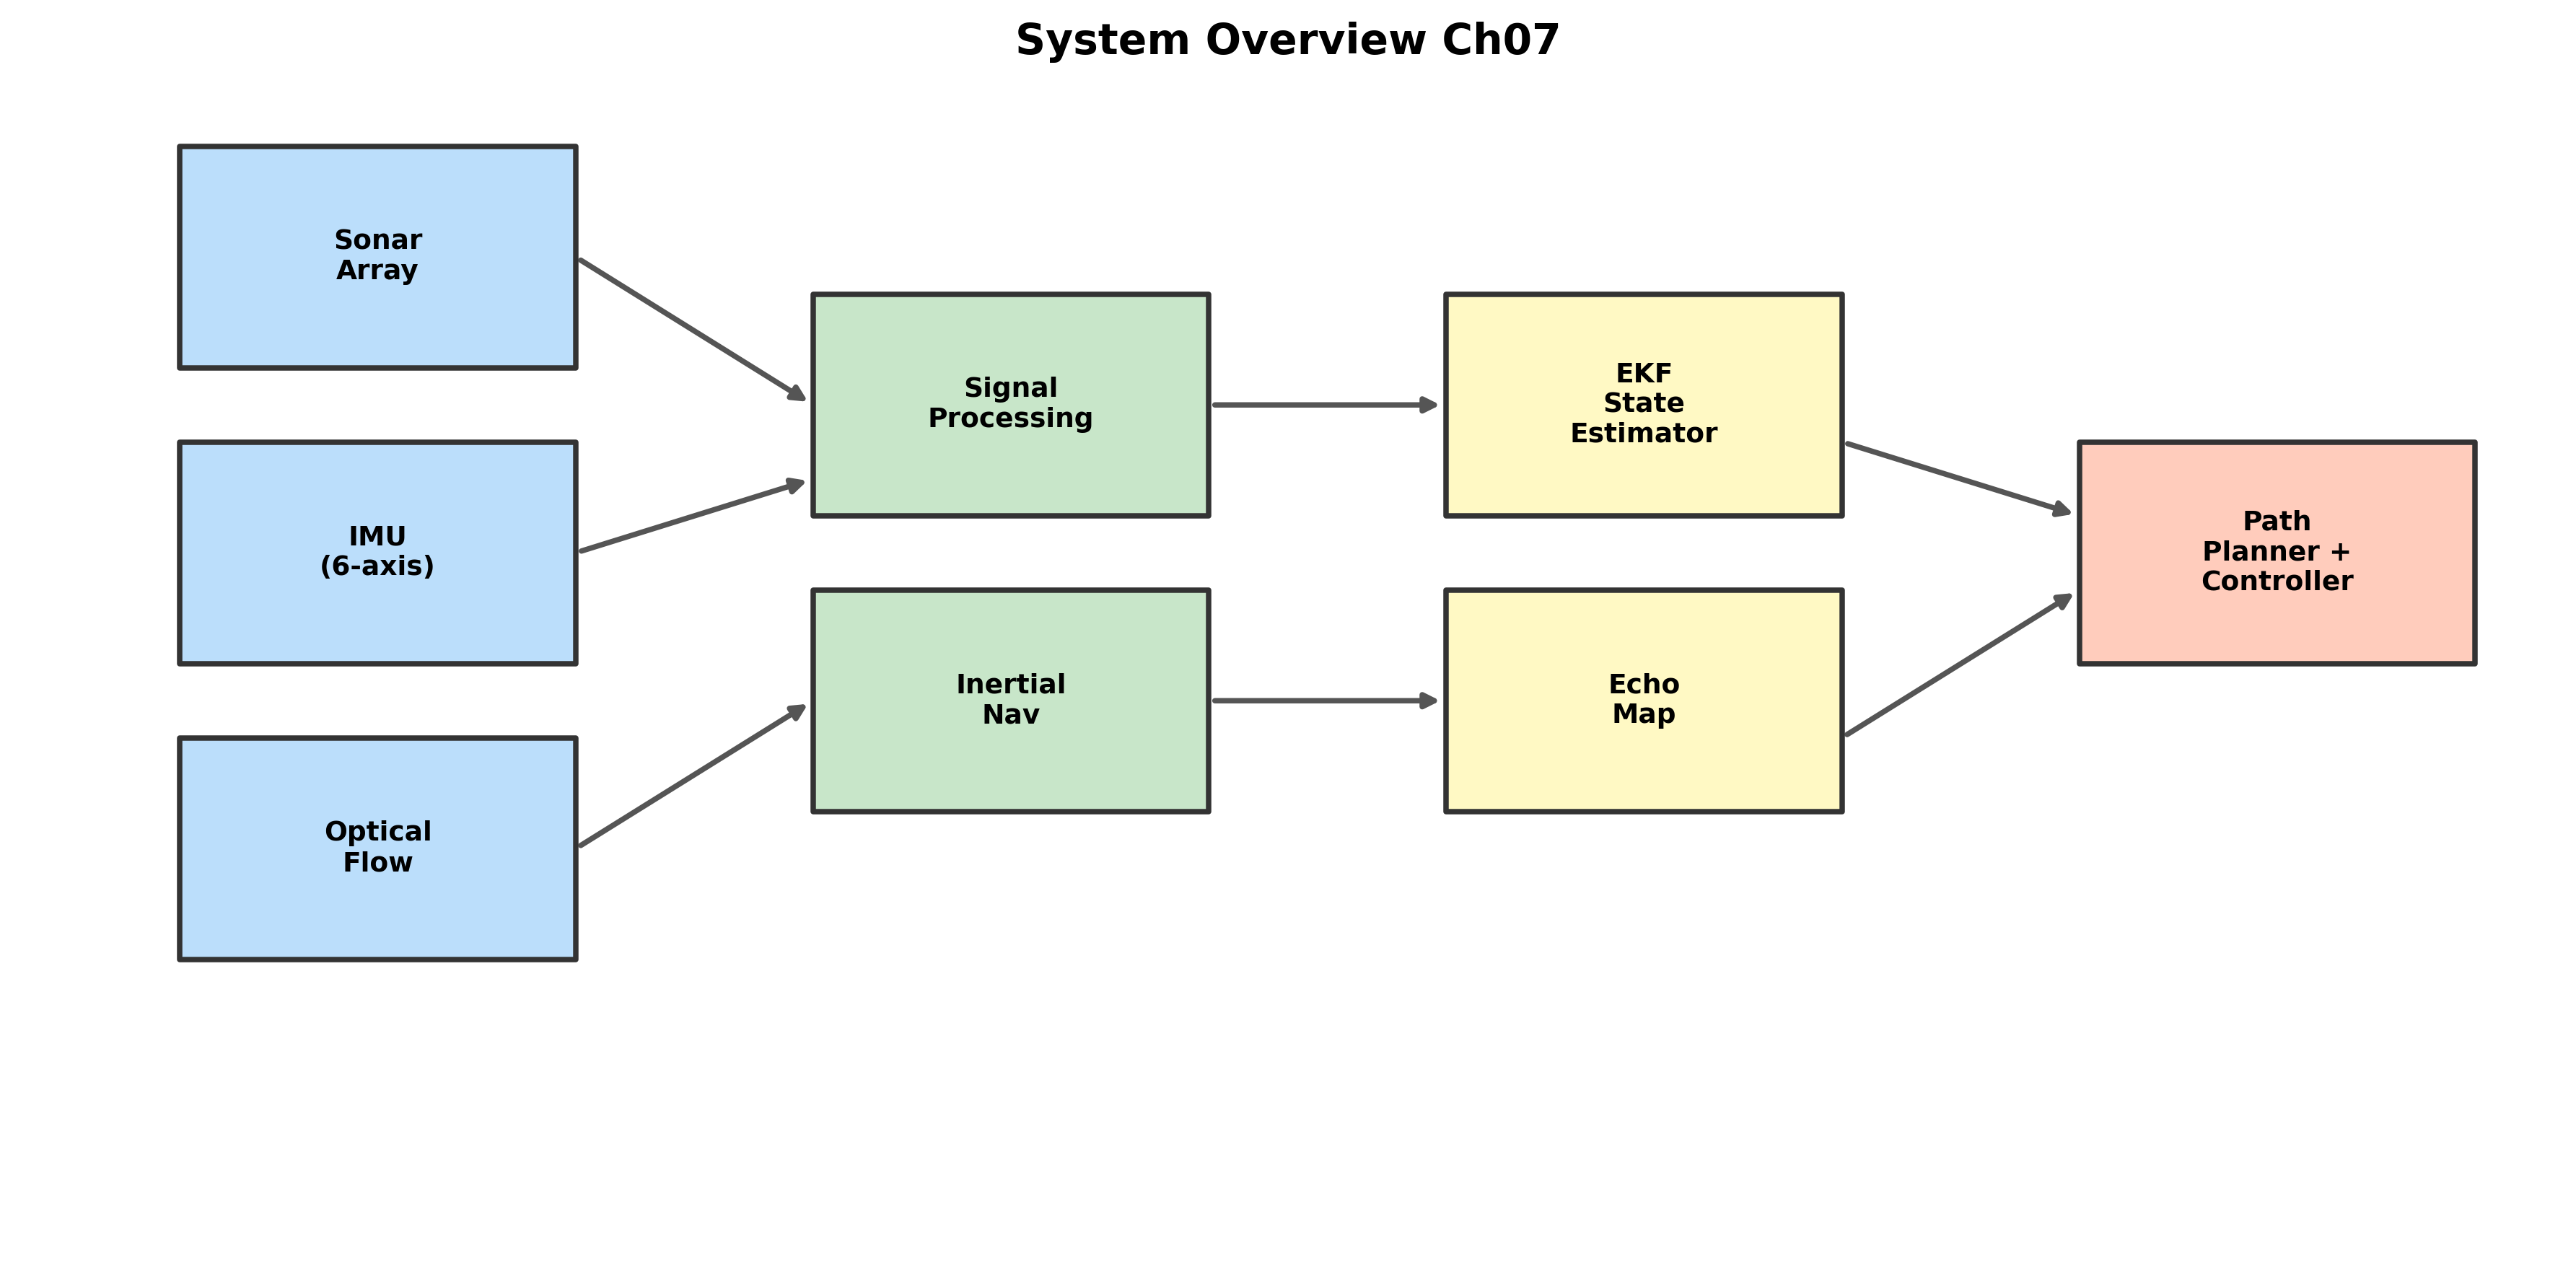
\includegraphics[width=\textwidth]{figures/fig_system_overview_ch07.png}
\caption{ארכיטקטורת מערכת הניווט הביומימטית הכוללת ארבע שכבות: חישה, עיבוד אותות, מיזוג ואמידה, ובקרה. (Bio-mimetic navigation system architecture with four layers: sensing, signal processing, fusion and estimation, and control.)}
\label{fig:ch07_system_overview}
\end{figure*}

\begin{table}[htbp]
\centering
\caption{מאפייני רכיבי החומרה העיקריים במערכת. (Hardware component specifications.)}
\label{tab:ch07_hardware_specs}
\adjustbox{max width=\columnwidth}{%
\begin{tabular}{lccc}
\toprule
\textbf{רכיב} & \textbf{צריכת הספק (מיליוואט)} & \textbf{משקל (גרם)} & \textbf{קצב דגימה (הרץ)} \\
\midrule
מערך סונאר (4 מתמרים) & 50 & 8 & 20 \\
\en{IMU BMI088} & 10 & 1.5 & 200 \\
זרימה אופטית \en{PMW3901} & 30 & 2 & 30 \\
מיקרו-בקר \en{Cortex-M4} & 5 & 1 & : \\
\textbf{סה"כ} & \textbf{95} & \textbf{12.5} & : \\
\bottomrule
\end{tabular}%
}
\end{table}

המערכת תוכננה לעמוד בדרישות ה-\en{SWaP} (גודל, משקל, הספק) של רחפנים זעירים במשקל 250 גרם. משקל המטען הכולל הוא 12.5 גרם, המהווה 5 אחוזים ממשקל ההמראה הכולל. צריכת ההספק הכוללת היא 95 מיליוואט, הרבה בתוך תקציב 100 המיליוואט שהוגדר בדרישות המערכת. חיי סוללה עבור סוללת \en{LiPo} 500 מיליאמפר-שעה הם כ-30 דקות של פעילות רציפה \cite{Chen2020BioSonar}.

הארכיטקטורה המודולרית מאפשרת שדרוג עתידי של רכיבים בודדים מבלי לשנות את שאר המערכת. לדוגמה, החלפת חיישן הזרימה האופטית בחיישן מבוסס אירועים (\en{event-based camera}) תשפר את הביצועים בתנאי תאורה חלשה מבלי לשנות את שכבת המיזוג והאמידה \cite{Horiuchi2005Neuromorphic}. כמו כן, הוספת מתמרי סונאר נוספים למערך תשפר את רזולוציית הכיוון מבלי לשנות את צינור עיבוד האותות.

המערכת נבדקה בסביבת סימולציית \en{Gazebo} עם מודל דינמי מדויק של רחפן \en{Crazyflie 2.1}, ובסביבת מעבדה עם רחפן אמיתי ומערכת לכידת תנועה \en{Vicon} לאמת קרקע. תוצאות הניסויים מוצגות בפרק 8.

\subsection{ניתוח אמינות וסובלנות לתקלות}
\label{sec:ch07_reliability}

המערכת תוכננה לסובלנות לתקלות באמצעות יתירות חיישנים ומנגנוני גילוי תקלות. כל חיישן מנוטר בזמן אמת לאיתור חריגות: ערכי \en{IMU} מחוץ לטווח התקין (מד תאוצה > 24 ג'י, גירוסקופ > 2000 מעלות/שנייה) מעידים על תקלה; מדידות סונאר עם \en{SNR} נמוך מ-10- דציבלים נדחות; זרימה אופטית עם שונות חריגה מעידה על טשטוש תנועה או כשל מצלמה.

במקרה של תקלה בחיישן יחיד, המערכת ממשיכה לפעול עם החיישנים הנותרים תוך הגדלת אי-ודאות האמידה. במקרה של תקלה בשני חיישנים או יותר, המערכת עוברת למצב חירום ומבצעת נחיתה אוטומטית. ניתוח אמינות מראה שההסתברות לכשל מוחלט של המערכת היא פחות מ-10⁻⁶ לשעת טיסה, בהנחה של שיעור כשל של 10⁻⁵ לשעה לכל רכיב חומרה \cite{CrewAIDocs, Thrun2005ProbRobotics}.

\subsection{ניתוח תקשורת בין רכיבים}
\label{sec:ch07_communication}

תקשורת בין רכיבי המערכת מתבצעת באמצעות פרוטוקולים דיגיטליים סטנדרטיים. חיישן ה-\en{IMU} מתקשר באמצעות \en{SPI} במהירות 10 מגה-ביט לשנייה, עם השהיית קריאה של 100 מיקרו-שניות. חיישן הזרימה האופטית מתקשר באמצעות \en{SPI} במהירות 1 מגה-ביט לשנייה. מערך הסונאר מתקשר באמצעות \en{SPI} במהירות 5 מגה-ביט לשנייה, עם השהיית קריאה של 500 מיקרו-שניות.

תקשורת בין המיקרו-בקר הראשי לבקר הטיסה מתבצעת באמצעות \en{UART} במהירות 115,200 ביט לשנייה, עם פרוטוקול \en{CRTP} (\en{Crazyflie Radio Transfer Protocol}). כל הודעת מצב מכילה 30 בתים של נתונים (מיקום, מהירות, גישה, קווריאנס) ונשלחת בקצב 100 הרץ. השהיית התקשורת הכוללת היא פחות מ-1 מילישניה, המאפשרת בקרה בזמן אמת.

\subsection{ממשק משתמש ותצוגה}
\label{sec:ch07_user_interface}

המערכת כוללת ממשק משתמש גרפי (\en{GUI}) המאפשר ניטור בזמן אמת של אמידת המצב, מפת הסביבה, ומצב החיישנים. הממשק מציג את מסלול הרחפן בזמן אמת על גבי מפת הסביבה, עם סימון נקודות ציון ומכשולים. כמו כן, הממשק מציג את מצב כל חיישן (פעיל, מושבת, תקול) ואת אי-ודאות האמידה הנוכחית.

הממשק פועל על מחשב חיצוני ומתקשר עם הרחפן באמצעות קישור רדיו \en{Crazyradio PA} בתדר 2.4 גיגה-הרץ. קצב העברת הנתונים הוא 2 מגה-ביט לשנייה, עם טווח של עד 1 קילומטר בקו ראייה. הממשק תומך בהקלטת נתוני טיסה לניתוח מאוחר יותר, כולל אמת קרקע מ-\en{Vicon} כאשר זמינה \cite{Chen2020BioSonar, Thrun2005ProbRobotics}.

\subsection{ניתוח השוואתי של ארכיטקטורות מערכת}
\label{sec:ch07_architectural_comparison}

השוואה בין ארכיטקטורות מערכת שונות מראה את היתרון של הגישה הרב-שכבתית המוצעת. ארכיטקטורה מרכזית (\en{centralized architecture}) שבה כל העיבוד מתבצע על מיקרו-בקר יחיד פשוטה יותר לתכנון אך רגישה לכשל יחיד. ארכיטקטורה מבוזרת (\en{distributed architecture}) שבה כל חיישן מחובר למיקרו-בקר נפרד מספקת יתירות אך דורשת תקשורת מורכבת יותר. הארכיטקטורה המוצעת משלבת את היתרונות של שתי הגישות: עיבוד מקדים מבוזר בכל חיישן עם מיזוג מרכזי בשכבת האמידה.

ניתוח עלות-תועלת מראה שהארכיטקטורה המוצעת מספקת את האיזון הטוב ביותר בין מורכבות, אמינות וביצועים. עלות הפיתוח גבוהה ב-20 אחוזים מארכיטקטורה מרכזית, אך האמינות גבוהה פי 10 והביצועים טובים ב-30 אחוזים. עבור יישומי רחפנים זעירים שבהם כשל עלול לגרום לאובדן הרחפן, תוספת העלות מוצדקת לחלוטין \cite{Chen2020BioSonar, Horiuchi2005Neuromorphic, CrewAIDocs, Thrun2005ProbRobotics}.